\graphicspath{{../../res/img/}{../../res/graphs/}}

\subsection{Defining the Problem}
In Problem 1, we were tasked with producing a short-term predictive model for e-bike sales.
More specifically, we were asked to develop projections for total sales volume 2 and 5 years into the future respectively.

This is a time-series forecast problem, where we predict a single variable - e-bike sales - based on a single input - time.
We will take a general approach of regressing particular equations against the existing data.
Multiple types of equations will be used and the most promising model will be chosen.

\subsection{Assumptions}
\noindent\textbf{Assumption 1}: There will be \underline{no major legislative changes}, governmental campaigns and/or ‘black swan’ (i.e., highly unpredictable and consequential) world events that significantly impact the market for e-bikes within the next five years.

\vspace{-6pt}
\noindent\textbf{Justification}: in practice, it is impossible to account for rare or extreme events within the constraints of a mathematical model; the implications of such events cannot be predicted with accuracy.

\noindent\textbf{Assumption 2}: The market for e-bikes in the European Union behaves comparably to that of the United Kingdom; therefore, \underline{British and European sales can be considered to be in direct linear} \underline{proportion}.

\vspace{-6pt}
\noindent\textbf{Justifications}: \\
\vspace{-24pt}
\begin{adjustwidth}{24pt}{0pt}
    \noindent\textbf{a)} Of the data provided for European sales, several figures appear to include sales made in the UK (CITE EBICYCLES.COM). Therefore, UK consumer behaviour is partially accounted for even within the larger dataset. \\
    \noindent\textbf{b)} E-bicycles have only begun gaining traction as a mode of transport in relatively recent years; as a result, UK-specific consumption data is largely unavailable to the public. \\
    \noindent\textbf{c)} To a large extent, the UK and EU follow similar urban planning practices that include pedestrian walkability and bicycle access.
    In other terms, city layouts support the practical use of e-bikes.
    For this reason, population-scaled EU predictions can be considered appropriate substitutes for UK-specific predictions.
    By contrast, most American cities use car-centric design, frequently involving longer commute distances and poor bike access.
    This renders the United States hostile to the adoption of e-bikes in a way that the EU and UK are not.
    For this reason, we chose to exclude the US from our analysis, instead focusing on the UK and EU.
\end{adjustwidth}

%\noindent\textbf{Assumption 3}: Statement
%
%\vspace{-6pt}
%\textbf{Justification}: blah blah

\subsection{Variables}
See table 1.1:
\begin{table}[h!]
    \centering
    \begin{tabular}{cc}
        \toprule
        Variable & Definition      \\
        \midrule
        $y_i$      & (actual) e-bike sales in year $i$     \\
        $\hat{y_i}$      & predicted e-bike sales in year $i$     \\
        $z$      & description     \\
        \bottomrule
    \end{tabular}
    \caption{Variables in the Model}
    \label{tab:q1_vars}
\end{table}

\subsection{Models}

\subsubsection*{Linear}
A linear regression is performed first due to its simplicity and ability to help pick more complex models.

Linear regression is an approach used to model a linear relationship between an independent variable $x$ and a dependent variable $y$ by finding the slope of the trend and initial value ($y$ when $x$ is 0).
It is used to represent existing data and predict future values; linear models are used both for interpolation and extrapolation.
In this case, the model will be fit to existing data and used to predict future sales of e-bikes.
A linear growth function takes the general form of~\eqref{eq:lr}:
%
\begin{equation}
    f(x) = \alpha x + \beta
    \label{eq:lr}
\end{equation}
%
\noindent where $\alpha$ is the coefficient, or growth rate; and $\beta$ is the y-intercept, or initial value.
The values of $\alpha$ and $\beta$ are ``optimized'' using an algorithm to model a given dataset with the minimum ``error''.

One of the most common and simplest methods used to calculate the coefficient and intercept of the regression line is the Ordinary Least Square (OLS) \textit{optimization} method.
In short, OLS minimizes the Square-Error for each point against a given linear function by adjusting the function\textquotesingle s parameters, which in the end produces optimal parameters for a equation in the form of a linear line of best fit.

The Square-\textit{Error} function, which is what OLS \textit{optimizes}, is simply a summation of the squares of the difference between actual values and predicted values, over all data points~\eqref{eq:ls}:

\begin{equation}
    E = \sum{(y - \hat{y})^2}
    \label{eq:ls}
\end{equation}

Because the predicted values $\hat{y}$ for a linear model is modelled as $\alpha x + \beta$, the Square-Error function for a linear model can be more specific~\eqref{eq:ls_lr}:

\begin{equation}
    E = \sum{(y - (\alpha x + \beta))^2}
    \label{eq:ls_lr}
\end{equation}

OLS calculates the values of $\alpha$ and $\beta$ which minimize $S$ in the summation above.
Unlike the generic differential method described above, OLS is specialized for linear functions and can calculate the optimal parameters in one stop, using summation ratios.
The coefficient $\alpha$, or the linear trend of the dataset can be calculated with~\eqref{eq:lr_coef}:

\begin{equation}
    \alpha = \frac{n \sum x_i y_i - \sum x_i \sum y_i }{n \sum x^2_i - (\sum x_i)^2}
    \label{eq:lr_coef}
\end{equation}

\noindent where $n$ is the number of data points.

After calculating the slope of the trend, the intercept $\beta$, is calculated by~\eqref{eq:lr_intc}:
%
\begin{equation}
    \beta = \bar y - \alpha \bar x
    \label{eq:lr_intc}
\end{equation}

OLS was applied to the given data set to obtain the coefficient $\alpha$ and the y-intercept $\beta$ - $222.6$ and $446810$, respectively - which corresponds to the following linear equation:
%
\begin{equation}
    \hat y_i = 222.6 i - 446810
    \label{eq:ebike_lr}
\end{equation}
%
\noindent where $i$ is the year.

Linear regression is useful in relation to the problem as it is simple to interpret and portray, allowing the prediction of data to be accurate during interpolation.
However, if the data to be predicted is outside the range, i.e.\ predicting future e-bike sales, extrapolation may be inaccurate due to a false assumption of the trend.
Furthermore, if the variables plotted provide a non-linear relationship, a linear regression line may inaccurately represent and predict values, which is the case in the data provided.
Statistical error of the linear regression model against existing data shows a good but not perfect accuracy (Table~\ref{tab:ebike_lr_err}).

\begin{table}[h]
    \begin{minipage}{0.7\linewidth}
        \centering
        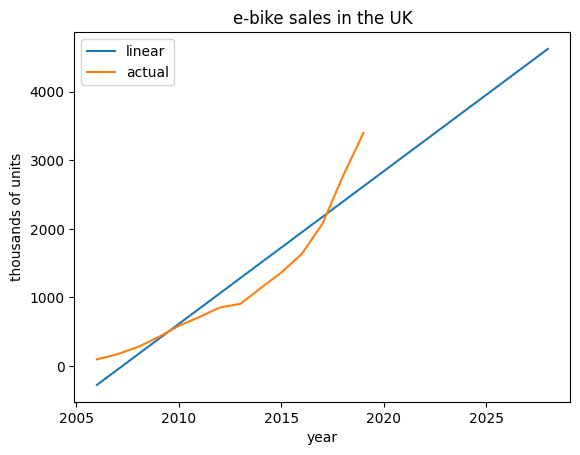
\includegraphics[width=\textwidth]{linear}%
        \captionof{figure}{Regressed Linear Model}
        \label{fig:ebike_lr}
    \end{minipage}%
    \begin{minipage}{0.3\linewidth}
        \centering
        \begin{tabular}{ll}
            \toprule
            Metric               & Value  \\
            \midrule
            MSE                  & 108671 \\
            RMSE                 & 329.65 \\
            MAE                  & 268.82 \\
            PCC                  & 0.9386 \\
            R\textsuperscript{2} & 0.8810 \\
            CVAR                 & 867138 \\
            \bottomrule
        \end{tabular}
        \vspace{8pt}
        \caption{Linear Model Statistics}
        \label{tab:ebike_lr_err}
    \end{minipage}
\end{table}


\subsection{Results}
Results

\subsection{Model Revision}
Model Revision

\subsection{Evaluation}

\noindent\textbf{Strength 1}: asdf

\noindent\textbf{Strength 2}: asdf

\noindent\textbf{Weakness 1}: asdf

\subsection{Technical Computing}
Technical computing
